
\section{User Study}
\subsection{Piloting}


\subsection{Experiment Design}
We had a gender-matched, within-group experimental design for the user study and varied avatar appearance for each trial. Participants played five trials of rope-pulling with the five avatars chosen from the survey. The avatars were meant to display various degrees of strength and intimidation. We chose the weakest and strongest male and female avatars, and three equidistantly rated avatars in between. We present the values of the ratings in Section \ref{section:surveyResults}. If there were avatars with the same equidistant rating, we chose the one with the most unique design.  The avatars were randomized for each participant at the start of the experiment. This study was ran alongside another study by researchers within the department. We made a common call for participants to take part in a \textit{VR Games Study}. Their task was to assess to virtual reality games and give researchers their feedback. The two games were Tug-of-war VR and a Whack-a-mole VR. At the end of the experiment, participants had a short recorded chat with the experimenter about their experience.

\subsection{Setup and Measurements}
For the experiment we used a Predator Helios 300 Acer laptop with an Nvidia GeForce GTX 1060, VRREADY graphics card. VE immersion was achieved by using a HTC Vive headset with a resolution of 2160x1200 and a refresh rate of 90Hz. 
Players' hand movements were tracked by the Noitom HI5 Vive tracker gloves\footnote{https://hi5vrglove.com/}. The glove uses a wrist-mounted Vive tracker to generate users' presumed hand position. 
We measure the force of participants' pulling through a digital force  with a seven-segment display. The force meter was fastened inside a box and placed on a table. We recorded the force by filming the digital display with a Intel RealSense VF0800 Developer Kit Digital Depth Camera\footnote{https://www.intelrealsense.com}.
To hide the measuring mechanism and increase ambiguity, participants pulled a rope between two black sheets which hid the whole set up of the experiment. This setup is shown in \ref{fig:setupBlack}. The force meter was placed on a table and it was tied to a heavy piece of furniture. So that participants would not hear the sound of a boxed hitting a table when lifting the rope, a piece of cloth was placed under the box. Various amortizing materials were placed inside the box to absorb sound and prevent the force meter from being damaged. The rope was tied to an elastic cable connected to a strong spring. The spring was connected to the force meter. The elastic band offered less resistance and, as participants pulled, the spring increased resistance. This spring mechanism was designed to increase realism and offer users some resistance in order to give the impression of a force acting on the rope. The box and spring mechanism can be see in figures \ref{fig:setupRopeBox1} and \ref{fig:setupRopeBox2}.\\


\begin{figure}[h]
  \centering
  \hfill
  \begin{minipage}[b]{0.4\textwidth}
    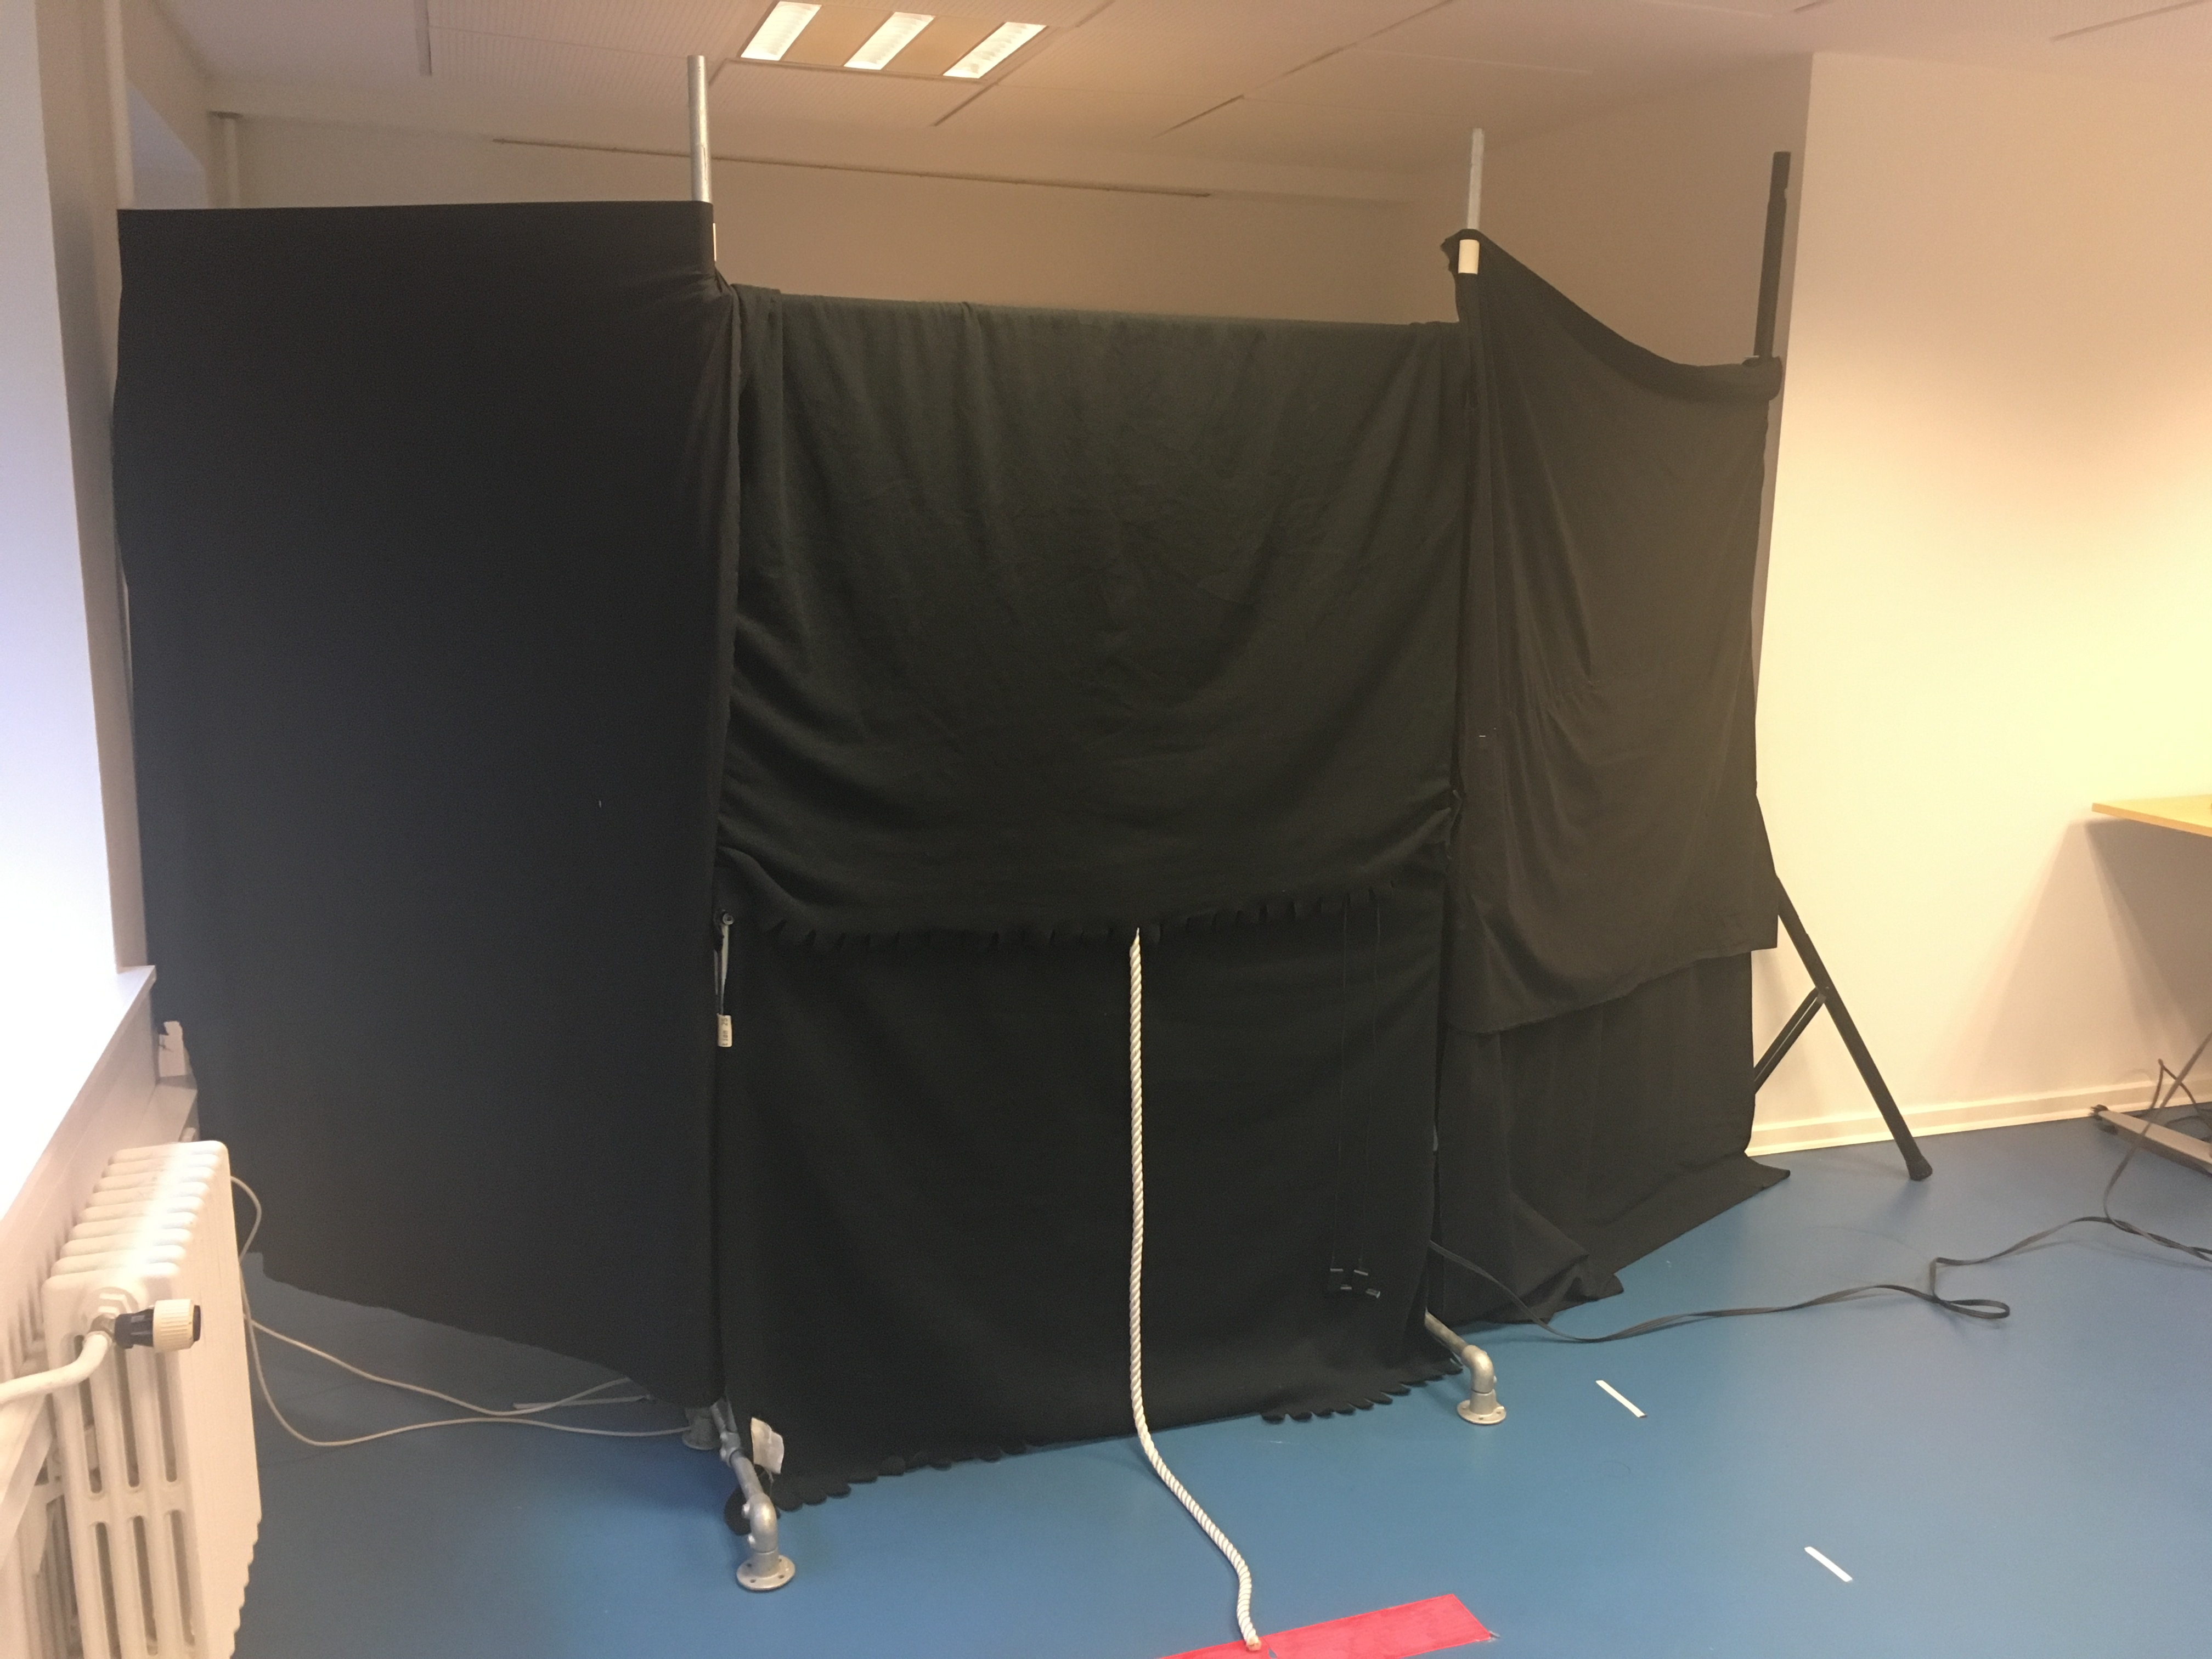
\includegraphics[width=\textwidth]{Images/setup1.JPG}
  \end{minipage}
  \hfill
  \begin{minipage}[b]{0.4\textwidth}
    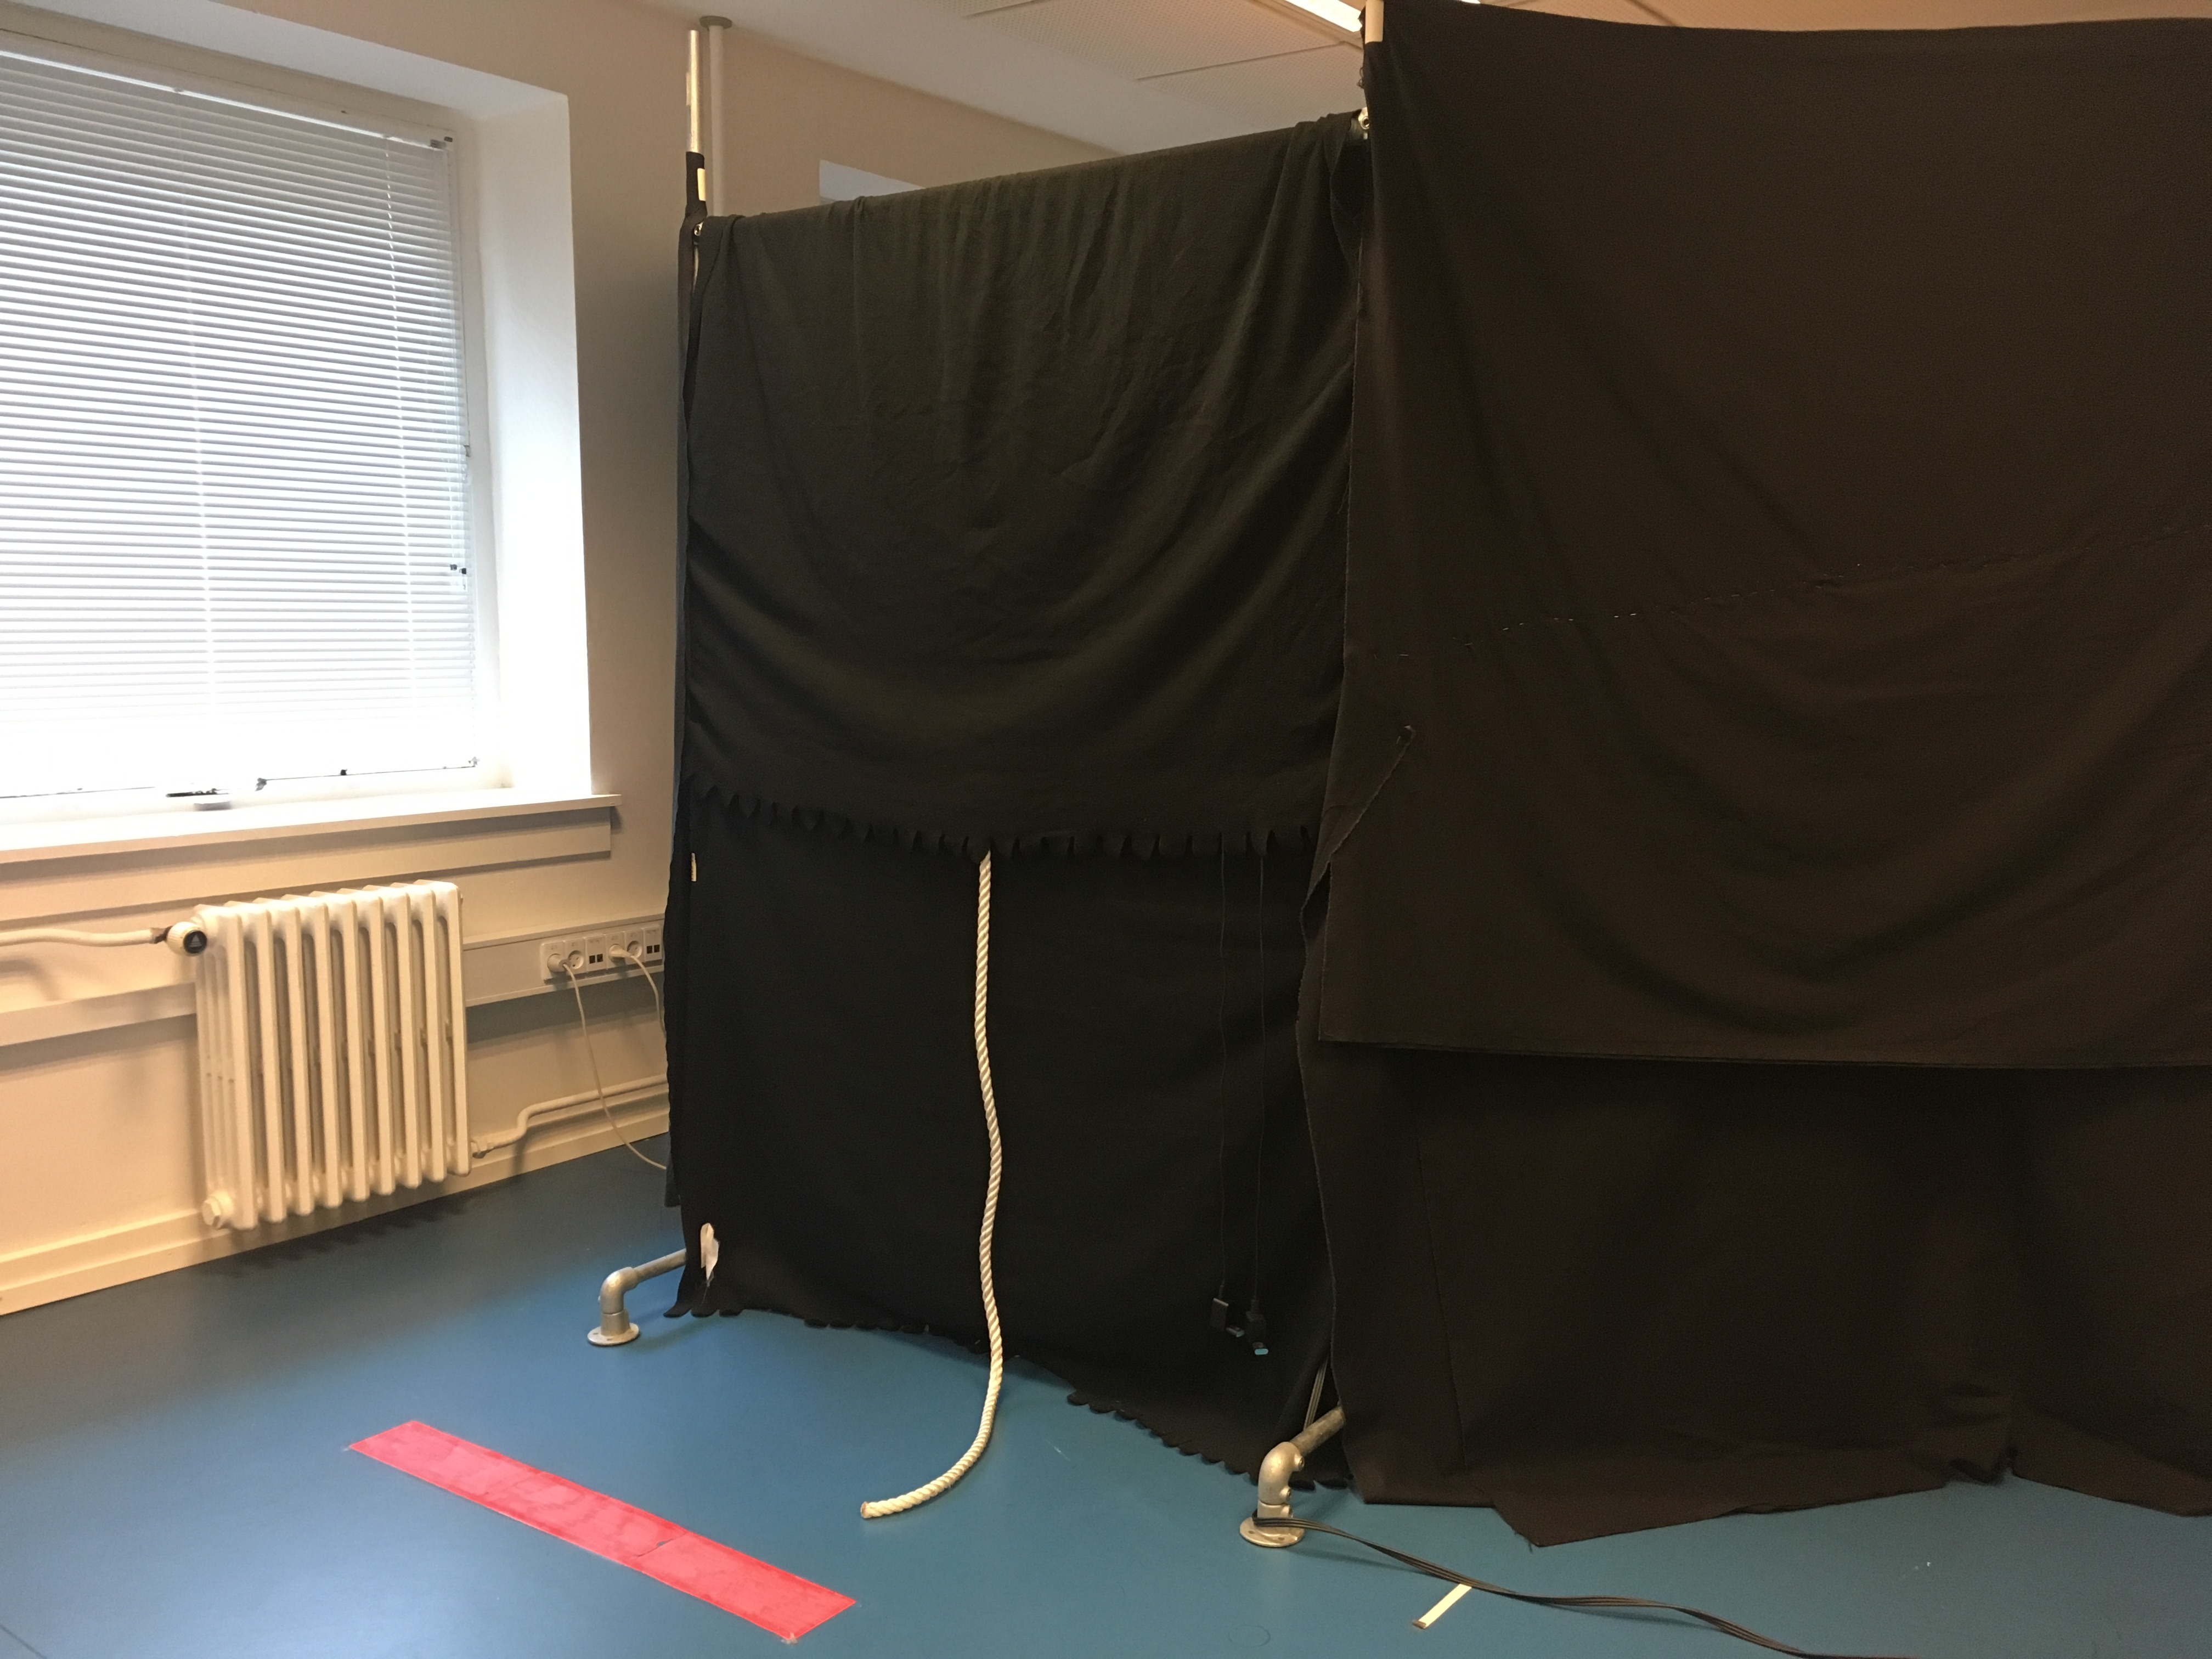
\includegraphics[width=\textwidth]{Images/setup2.JPG}
  \end{minipage}
  \hfill
     \caption{Participants' view of the setup.}
     \label{fig:setupBlack}
\end{figure}

\begin{figure}[H]
  \centering
  \hfill
  \begin{minipage}[b]{0.4\textwidth}
    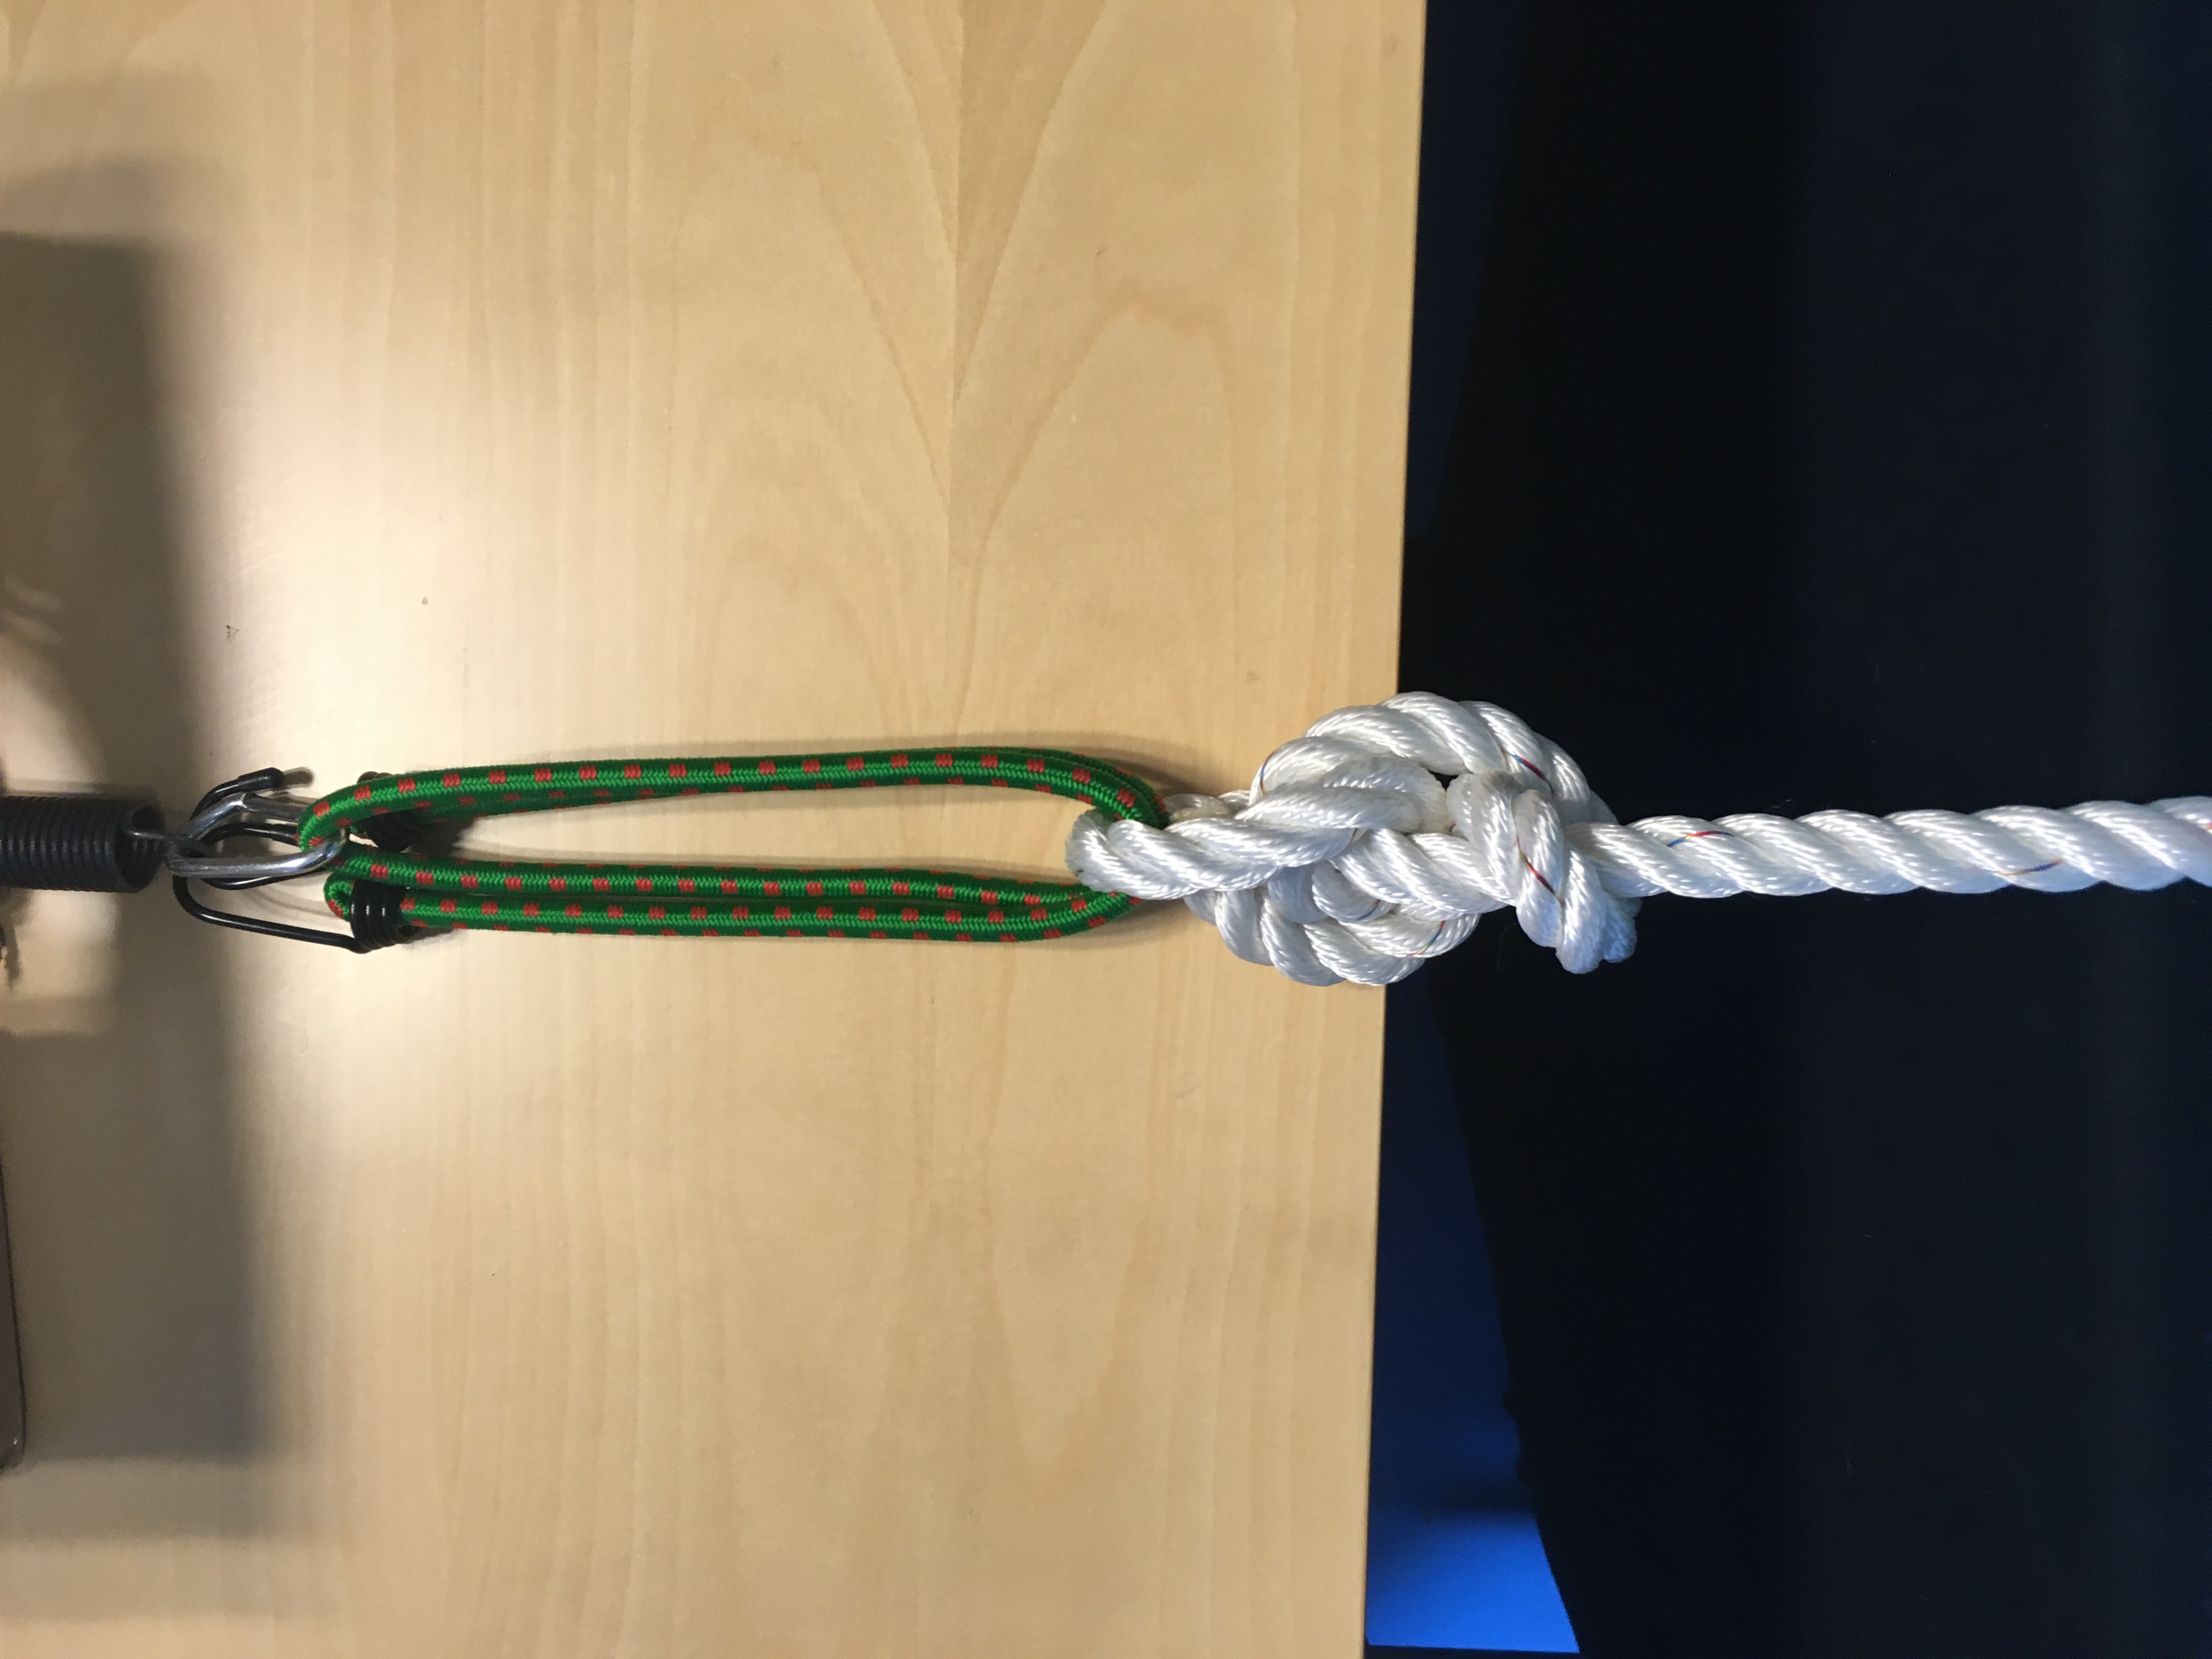
\includegraphics[width=\textwidth]{Images/rope.JPG}
    \caption{Rope and spring tied to the meter.}
     \label{fig:setupRopeBox1}
    \end{minipage}
  \hfill
  \begin{minipage}[b]{0.4\textwidth}
    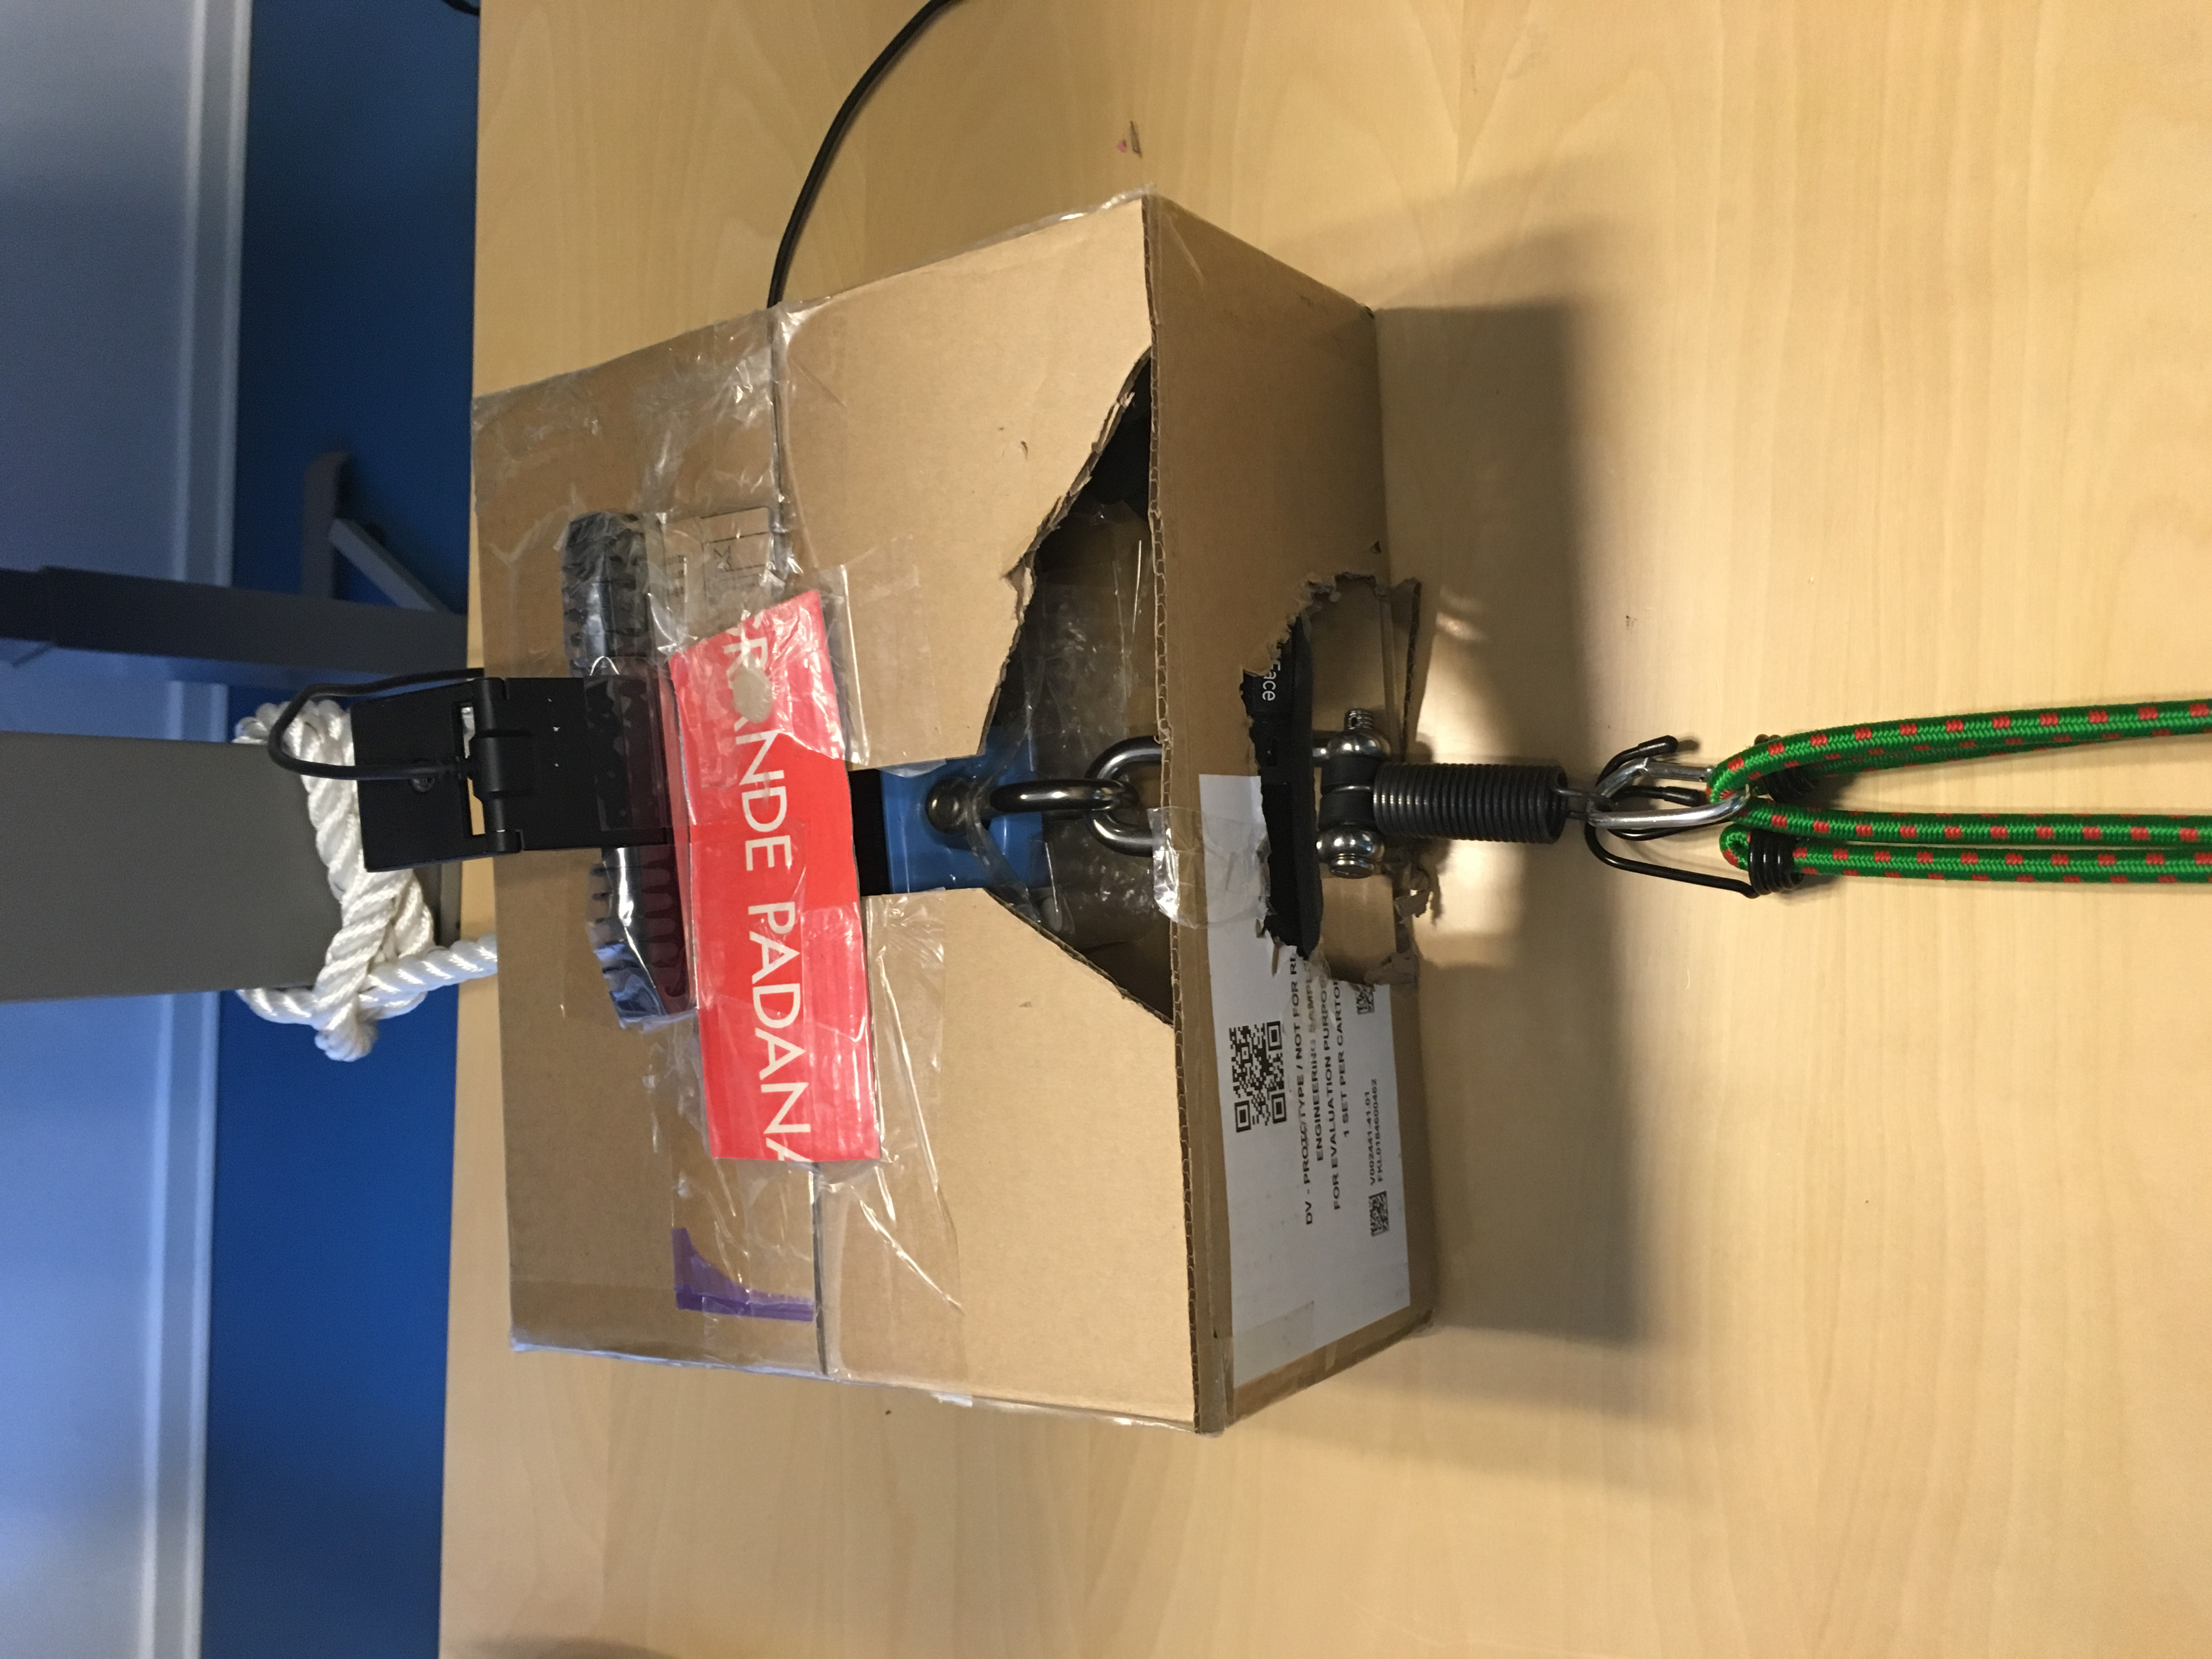
\includegraphics[width=\textwidth]{Images/BoxBig.JPG}
    \caption{Box with force meter and camera.}
     \label{fig:setupRopeBox2}
  \end{minipage}
  \hfill
    
\end{figure}



\subsection{Procedure}
Between each trial, participants answered the following questions from withing the VE. They were told to read the questions out loud and give their answers to the experimenter.  \todo{add pic of QPANEL} 

Afterwards we conduct a survey in which participants rate the self-perceived force they had for each condition, and how much they felt their opponents pulled. We also measure how strong they think each opponent looked. 

At the end we ask about the participant’s experience with the game in a short 2 minute interview and if they have any suggestions to improve it. Finally we ask the participants what they think the purpose of this experiment was in order to discard participants who showed a high awareness of the experimental aim. In the end we debrief users and tell them about the intended purpose of the experiment.
 ipq and other survey dataafter
\subsection{Results}
\subsubsection{Quantitative Results}
\subsubsection{Qualitative Observations}


\subsection{Discussion}

\subsection{Limitations}
- spring absorbs force a participant streched the spring too much and it was replaced